\documentclass[a4paper, 12pt]{article}
\usepackage[a4paper, margin=1in]{geometry}      % customize layout
\usepackage{mathptmx}
\usepackage[T1]{fontenc}                        % enhance fonts
\usepackage[utf8]{inputenc}                     % special characters are usable now
\usepackage{microtype}                          % provides smooth text appearance and auto hyphenation
\usepackage{indentfirst}                        % indent after new section
\usepackage[english]{babel}                     % document language is english
\usepackage{mathtools}                          % rearranges the equations display geometry
\usepackage{paralist}                           % compact lists, customizable labels and layout options
\usepackage{graphicx}                           % include graphicals
\usepackage[section]{placeins}                  % causes an implicit \FloatBarries to be used at the beginning of each section, so figure dont float into another section
\usepackage{wrapfig}                            % lets text flow around a figure or a table: environments: wrapfigure, wraptable
\usepackage{bookmark}                           % some support type thing
\usepackage{hyperref}                           % bookmarking
\usepackage{varioref}                           % introduces the functions \vref and \vpageref, smart \ref and \pageref
\usepackage{cleveref}                           % introduces the functions \cref, \crefrange, \cpageref, \cpagerefrange
\hypersetup{pdfauthor={Ali Ucar},
  pdftitle={Experiment 2 Prereport},
  pdfsubject={Capturing Rectilinear and Planar Motion},
  pdfkeywords={kinematics, motion, capture, experiment}}

\makeatletter
\renewcommand\@seccntformat[1]{}
\makeatother
\newcommand{\head}[1]{\section{\normalsize \textit #1}}
\newcommand{\subhead}[1]{\subsection{\normalsize #1}}

\begin{document}
    \title{Exp. 2: Capturing Rectilinear and Planar Motion}
    \author{Ali Uçar}
    \date{\today}
    % \maketitle
    \noindent
    \textbf{Name Surname:} Ali Uçar
    \hfill
    \textbf{Date:} \today \\
    \textbf{Student ID No:} 255555 \\
    \textbf{Section No:} 1 - Lab. Sec. 6

    \begin{center}
        \head{Exp. 2: Capturing Rectilinear and Planar Motion}
    \end{center}

    \subhead{Experiment Background and Theory}
    In this experiment, the local gravity will be measured by noting time intervals of a falling body until it
    reaches the floor. Where the local acceleration parameter is equal to the gravity in this experiment,
    measurements of the change in time intervals and positions of the falling body will be noted, then the
    local gravity will be calculated. Derived calculations will substitute local gravity.

    \begin{equation}
        v_i = \frac{y_{i+1} - y_i}{\Delta t}
    \end{equation}

    For time intervals of each frame $\Delta t$ is constant, corresponding successive locations related to 
    acceleration is shown below.

    \begin{equation}
        a_j = \frac{v_{j+1} - v_j}{\Delta t} = \frac{\frac{y_{i+2}-y_{i+1}}{\Delta t} - \frac{y_{i+1}-y_{i}}{\Delta t}}{\Delta t} =
        \frac{y_{i+2}-2y_{i+1}+y_i}{{\Delta t}^2} = a_{i \rightarrow i+2}
        \label{eq:accel}
    \end{equation}

    \bigskip \noindent

    \subhead{Description of Experiment \& Drawings or Sketches of Setup}
    \begin{wrapfigure}{l}{0.25\textwidth}
        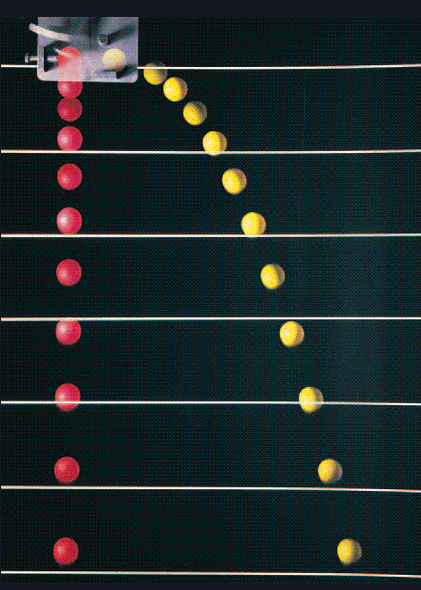
\includegraphics[width=0.20\textwidth]{./fall.png}
        \caption{Free-falling model of a particle}
    \end{wrapfigure}

    The local gravity where the experiment takes place will be measured by 
    recording a falling body in one-dimensional motion and dividing the time it took 
    for to fall into finite intervals, one interval being one frame, where the recorder 
    device capture at a rate of 60 FPS. For task A of this experiment, the falling body 
    is a ball. The digital software Tracker will be used to parameterize the one-dimensional 
    motion. A table of data sets will be noted, including the parameters 
    time, height, velocity, and acceleration. Then, a plot of sampled velocities vs. time
    graph will be illustrated as to show the acceleration is constant. For part B of the 
    experiment, the same software will be used to analyze the motion of a ball which 
    creates a two-dimensional shape. From the task B, the shape of a two-dimensional
    motion will be made sure that it is a parabola. Then, all the usual suspect 
    parameters in \cref{eq:accel} will be extracted.

    \subhead{References}
    \url{https://www.compadre.org/precollege/items/detail.cfm?ID=10001}

    \clearpage
\end{document}

